\chapter{Mengenal Kecerdasan Buatan dan Scikit-Learn}
Buku umum yang digunakan adalah \cite{russell2016artificial} dan  
untuk sebelum UTS menggunakan buku \textit{Python Artificial Intelligence Projects for Beginners}\cite{eckroth2018python}.
Dengan praktek menggunakan python 3 dan editor anaconda dan library python scikit-learn.
Tujuan pembelajaran pada pertemuan pertama antara lain:
\begin{enumerate}
\item
Mengerti definisi kecerdasan buatan, sejarah kecerdasan buatan, perkembangan dan penggunaan di perusahaan
\item
Memahami cara instalasi dan pemakaian sci-kit learn
\item
Memahami cara penggunaan variabel explorer di spyder
\end{enumerate}
Tugas dengan cara dikumpulkan dengan pull request ke github dengan menggunakan latex pada repo yang dibuat oleh asisten riset.

\section{Teori}
Praktek teori penunjang yang dikerjakan :
\begin{enumerate}
\item
Buat Resume Definisi, Sejarah dan perkembangan Kecerdasan Buatan, dengan bahasa yang mudah dipahami dan dimengerti. Buatan sendiri bebas plagiat[hari ke 1](10)
\item
Buat Resume mengenai definisi supervised learning, klasifikasi, regresi dan unsupervised learning. Data set, training set dan testing set.[hari ke 1](10)
\end{enumerate}

\section{Instalasi}
Membuka https://scikit-learn.org/stable/tutorial/basic/tutorial.html. Dengan menggunakan bahasa yang mudah dimengerti dan bebas plagiat. 
Dan wajib skrinsut dari komputer sendiri.
\begin{enumerate}
\item
Instalasi library scikit dari anaconda, mencoba kompilasi dan uji coba ambil contoh kode dan lihat variabel explorer[hari ke 1](10)
\item
Mencoba Loading an example dataset, menjelaskan maksud dari tulisan tersebut dan mengartikan per baris[hari ke 1](10)
\item
Mencoba Learning and predicting, menjelaskan maksud dari tulisan tersebut dan mengartikan per baris[hari ke 2](10)
\item
mencoba Model persistence, menjelaskan maksud dari tulisan tersebut dan mengartikan per baris[hari ke 2](10)
\item 
Mencoba Conventions, menjelaskan maksud dari tulisan tersebut dan mengartikan per baris[hari ke 2](10)
\end{enumerate}


\section{Penanganan Error}
Dari percobaan yang dilakukan di atas, apabila mendapatkan error maka:

\begin{enumerate}
	\item
	skrinsut error[hari ke 2](10)
	\item
Tuliskan kode eror dan jenis errornya [hari ke 2](10)
	\item
Solusi pemecahan masalah error tersebut[hari ke 2](10)

\end{enumerate}


\section{Fathi Rabbani / 1164074}
\subsection{Teori}
\begin{enumerate}
\item
Sejarah dan Perkembangan Kecerdasan Buatan
\subitem
Sejarah dari sebuah Artificial Intelligence atau dalam Bahasa indonesianya diterjemahkan sebagai Kecerdasan Buatan adalah sebuah usaha untuk dapat memodelkan sebuah mesin agar dapat berfikir dan menirukan tingkah laku dan cara berfikir manusia, ada beberapa jenis dari kecerdasan buatan, yaitu :

\begin{itemize}
\item
Symbol Manipulating AI
\item
Nueral AI
\item
Neural Network
\end{itemize}
\subitem
Peneliti yang selalu disebutkan sebagai Bapak AI adalah Jhon McCharty  merupakan seorang dosen yang mengenalkan Kecerdasan Buatan kepada 2 lembaga penelitian hebat, yaitu Stanford Artificial Intelligence Laboratory dan MIT Artificial Intelligence Laboratory.
\subitem
Sedangkan perkembangan kecerdasan buatan saat ini sudah mencapai tahap dimana manusia mulai membuat sebuah robot yang dapat menirukan hampir 90 persen dari keseharian mereka, mulai dari bidang kesehatan, koki, pabrik, kantoran, hingga sebuah robot yang bertugas sebagai seorang pelayan di sebuah restoran. Dan dubai sebagai pengguna mobil tanpa pengemudi yang menerapkan AI dengan menggunakan data wilayah serta jarak kendaraan dengan pingir jalan.
\item
Definisi Supervised, Unsupervised Learning, Klasifikasi, Regresi serta Data, Training, Testing Set
\begin{itemize}
\item
Supervised learning merupakan sebuah pendekatan AI dengan latihan yang sudah dilakukan dengan sebuah data yang lengkap, dan memiliki variable yang dapat digunakan sebagai target sehingga dapat menujukan data agar menjadi kelompok dari sebuah data menjadi kelompok data yang baru.
\item
Unsupervised learning merupakan sebuah pendekatan AI tanpa menggunakan data yang lengkap dan ter-variable sehingga harus dilakukan pengelompokkan agar data tersebut dapat digunakan.
\item
Klasifikasi merupakan sebuah pengelompokkan suatu objek ke dalam kategori tertentu.
\item
Regresi merupakan pendekatan model matematika untuk mendeskripsikan hubungan dari beberapa variabel independen dengan variable dependen.
\item
Data Set, meupakan sebuah objek yang merepresentasikan data dan hubungannya di memory. 
\item
Training Set, subset untuk melatih model.
\item
Testing Set, subset untuk menguji model yang sudah dilatih.
\end{itemize}


\subsection{Praktikum}
\item
Instalasi Library Scikit dari Anaconda

\subitem
Pertama Download terlebih dahulu anaconda-nya di https://www.anaconda.com/distribution/ pilih Operating Sistem yang kalian gunakan. lalu setelah download Install dengan proses berikut :
\begin{itemize}
\item
Proses Instalasi Anaconda pada gambar \ref{proses2} hingga proses \ref{proses9}.
\item
Proses Instalasi Scikit-Learn dengan menggunakan Conda pada gambar \ref{proses10} hingga gambar \ref{proses12}.
\item
contoh dari Variable Explorer yang digunakan ada pada gambar \ref{proses14}.
\end{itemize}
\begin{figure}[ht]
\centerline{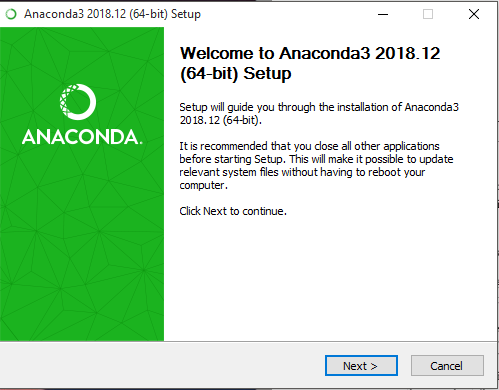
\includegraphics[width=1\textwidth]{figures/fathi/2.PNG}}
\caption{setelah membuka data instalasi klik next}
\label{proses2}

\centerline{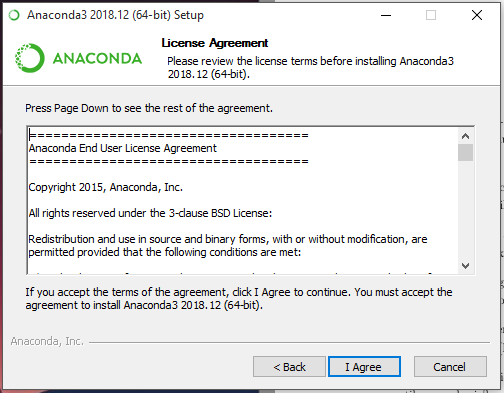
\includegraphics[width=1\textwidth]{figures/fathi/3.PNG}}
\caption{pilih i agree}
\label{proses3}
\end{figure}
\begin{figure}
\centerline{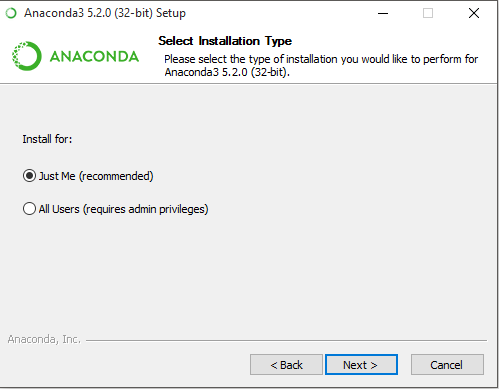
\includegraphics[width=1\textwidth]{figures/fathi/4.PNG}}
\caption{pilih instalasi Just Me}
\label{proses4}

\centerline{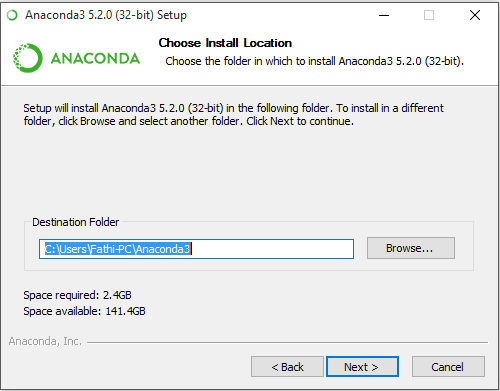
\includegraphics[width=1\textwidth]{figures/fathi/5.PNG}}
\caption{langsung saja next}
\label{proses5}
\end{figure}
\begin{figure}
\centerline{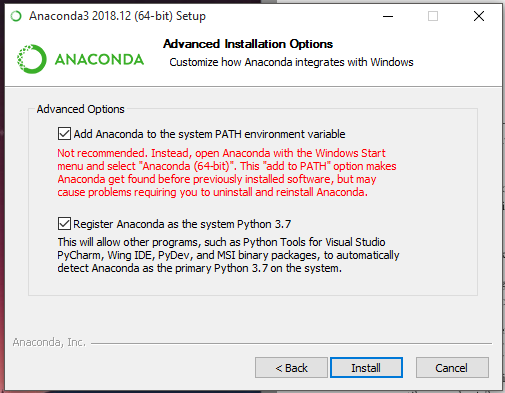
\includegraphics[width=1\textwidth]{figures/fathi/6.PNG}}
\caption{cek kedua pilihan tersebut}
\label{proses6}

\centerline{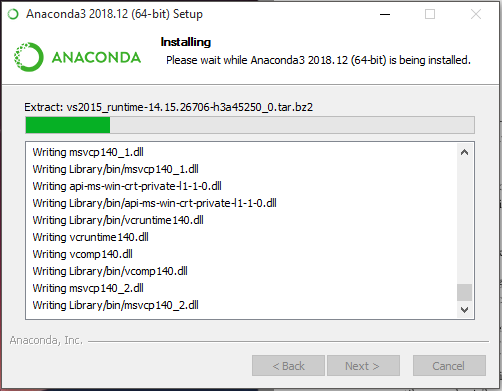
\includegraphics[width=1\textwidth]{figures/fathi/7.PNG}}
\caption{proses Instalasi}
\label{proses7}
\end{figure}
\begin{figure}
\centerline{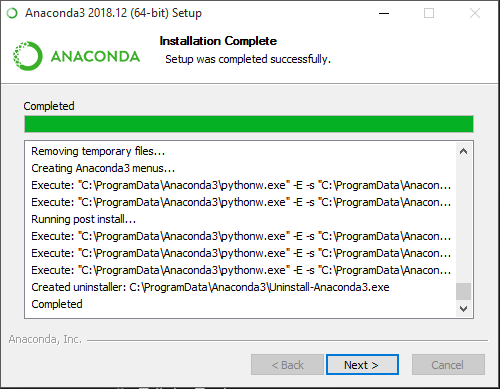
\includegraphics[width=1\textwidth]{figures/fathi/8.PNG}}
\caption{klik next}
\label{proses8}

\centerline{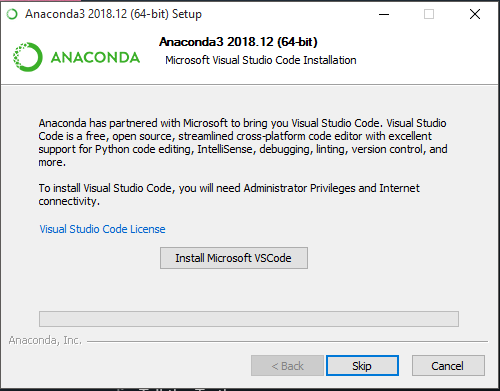
\includegraphics[width=1\textwidth]{figures/fathi/9.PNG}}
\caption{selesai instalasi anaconda}
\label{proses9}
\end{figure}
\begin{figure}
\centerline{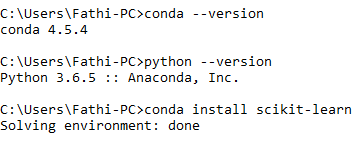
\includegraphics[width=1\textwidth]{figures/fathi/10.PNG}}
\caption{Instalasi SCIKIT dengan menggunakan anaconda}
\label{proses10}

\centerline{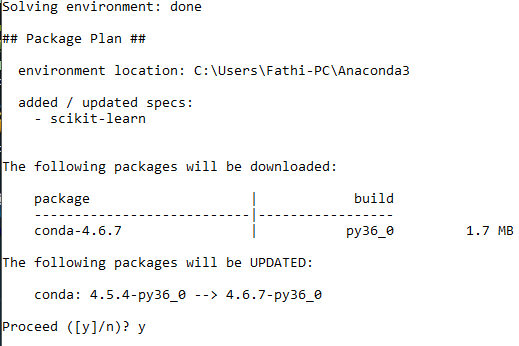
\includegraphics[width=1\textwidth]{figures/fathi/11.PNG}}
\caption{Konfirmasi Instalasi}
\label{proses11}
\end{figure}
\begin{figure}
\centerline{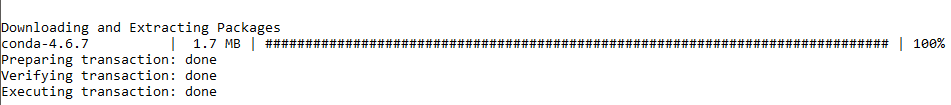
\includegraphics[width=1\textwidth]{figures/fathi/12.PNG}}
\caption{hasil dari instalasi SCIKIT}
\label{proses12}
\centerline{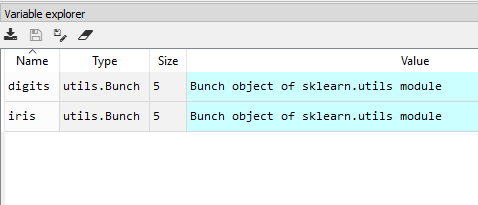
\includegraphics[width=1\textwidth]{figures/fathi/14.PNG}}
\caption{data variable explorer}
\label{proses14}
\end{figure}

\item
Load Example Dataset dan Menjeleaskan kegunakan barisan Code
\subitem
berikut ini adalah contoh dataset yang digunakan untuk melakukan compile ada pada gambar \ref{proses16} dan hasilnya ada pada gambar \ref{proses15}.

\begin{figure}
\centerline{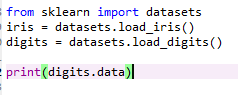
\includegraphics[width=1\textwidth]{figures/fathi/16.PNG}}
\caption{code example dataset yang digunakan}
\label{proses16}

\centerline{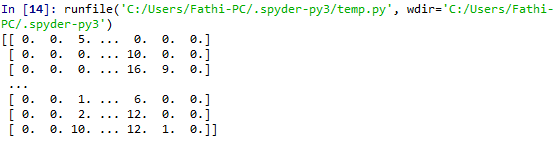
\includegraphics[width=1\textwidth]{figures/fathi/15.PNG}}
\caption{data hasil dari code example dataset yang digunakan}
\label{proses15}
\end{figure}
\begin{itemize}
\item
dari code yang dicoba diketahui bahwa data set yang digunakan adalah data yang diambil dari SKLEARN yang ada pada gambar \ref{proses16}.
\end{itemize}

\item
Learning and Predicting
\subitem
Dalam scikit-learn estimator untuk klasifikasi adalah sebuah objek data python yang memliki implementasi method fit(x, y) dan predict(T). Sebuah estimator danri class sklearn.svm.SVC,yang mana implemetasi dari support vector classification. Estimator dari konstruktor mengambil argument dari model parameter.
\begin{verbatim}
from sklearn import svm
clf = sv.SVC(gamma=0.001, C=100.)
clf.fit(digits.data[:-1], digits.target[:-1]
clf.predict(digits.data[:-1])
\end{verbatim}
\subitem
mengambil nilai data svm ada pada class sklearn, lalu set nilai data dengan clf = sv.SVC(gamma=0.001, C=100.). variable clf digunakan dengan method fit yang di set nilainya [:-1] yang memproduksi array baru dari data digits.data, dengan menggunakan digits.data sebagai acuan, sekarang tinggal melakukan prediksinya.

\item
Model Presistence

\begin{verbatim}
from sklearn import svm
from sklearn import datasets
clf = svm.SVC(gamma=0.001)
iris = datasets.load_iris()
X, y = iris.data, iris.target
clf.fit(X, y)
\end{verbatim}
\subitem
mengambil nilai data svm ada pada class sklearn dan mengambil nilai data datasets ada pada class sklearn, lalu buat variable clf dengan nilai data  dan buat variable yang berisi nilai load\_iris. variable X dan y yang berisi nilai iris data dan iris target, lalu memanggil nilai variable X dan y dengan data variable clf dan method fit.

\begin{verbatim}
import pickle
s = pickle.dumps(clf)
clf2 = pickle.loads(s)
clf2.predict(X[0:1])
y[0]
\end{verbatim}
\subitem
mengambil nilai data pickle dan membuat variable s dengan data nilai pickle.dumps yang berisi data variable clf, membuat variable clf2 dengan data pickle.loads yang menggunakan variable s. menggunakan data variable clf2 dengan method predict dengan data variable X dan data variable y.

\item
Conventions
\begin{itemize}
\item
\begin{verbatim}
import numpy as np
from sklearn import random_projection

rng = np.random.RandomState(0)
X = rng.rand(10, 2000)
X = np.array(X, dtype='float32')
X.dtype

transformer = random_projection.GaussianRandomProjection()
X_new = transformer.fit_transform(X)
X_new.dtype
\end{verbatim}
\subitem
mengambil data numpy dan dialiaskan sebagai np. dari data sklearn mengambil data random\_projection. lalu buat variable rng yang berisi nilai data np dengan random yang berawal 0. lalu variable X dengan data rng yang memiliki type rand berisi data 10 dan 2000. lalu dibuatkan arraynya dengan format X = np.array(X, dtype ='float32'). dan nilai variable transform yang digunakan untuk menampilkan hasil random, dengan format Gaussian random projection. format penampilannya X\_new = transformer.fit\_transform( X) dan X\_new.dtype

\item
\begin{verbatim}
from sklearn import datasets
from sklearn.svm import SVC

iris = datasets.load_iris()
clf = SVC(gamma=0.001)
clf.fit(iris.data, iris.target)

list(clf.predict(iris.data[:3]))

clf.fit(iris.data, iris.target_names[iris.target])

list(clf.predict(iris.data[:3])) 
\end{verbatim}
\subitem
dari data sklearn mengambil datasets dan SVC dari svm, selanjutnya membuat format data variable dengan nilai load\_iris\(\), clf dengan format SVC\(gamma=0.001\), lalu di jalankan dengan moethod clf.fit dengan iris.data dan iris.target sebagai nilainya.

buatkan tampilan datanya dengan list menampilkan data clf dengan predict pada iris.data, dan dilakukan selanjutnya dengan clf.fit dengan nilai data iris.data dan iris.target\_names[ iris.target]. tampilkan lagi dalam bentuk list data tersebut.

\item
\begin{verbatim}
import numpy as np
from sklearn.svm import SVC

rng = np.random.RandomState(0)
X = rng.rand(100, 10)
y = rng.binomial(1, 0.5, 100)
X_test = rng.rand(5, 10)

clf = SVC()
clf.set_params(kernel='linear').fit(X, y)

clf.predict(X_test)

clf.set_params(kernel='rbf', gamma=0.001).fit(X, y)

clf.predict(X_test)
\end{verbatim}
\subitem
mengambil data numpy dan dialiaskan sebagai np dan dari sklearn.svm mengambil data SVC,  lalu buat variable rng yang berisi nilai data np dengan random yang berawal 0, lalu variable X dengan data rng yang memiliki type rand berisi data(100, 10) dan y yang memiliki data (1, 0.5, 100) dengan type data binomial lalu buat X\_test untuk variable test.

\item
\begin{verbatim}
from sklearn.svm import SVC
from sklearn.multiclass import OneVsRestClassifier
from sklearn.preprocessing import LabelBinarizer

X = [[1, 2], [2, 4], [4, 5], [3, 2], [3, 1]]
y = [0, 0, 1, 1, 2]

classif = OneVsRestClassifier(estimator=SVC(gamma=1, random_state=0))

classif.fit(X, y).predict(X)

y = LabelBinarizer().fit_transform(y)
classif.fit(X, y).predict(X)
\end{verbatim}
\subitem
mengambil data sklearn SVC dari svm, OneVsRestClassifier dari multiclass, dan LabelBinarizer dari preprocessing. lalu buatkan variable X dan y yang berisi data nilai dan buatkan data variable classif untuk digunakan sebagai parameter bagi OneVsRestClassfier yang menghitung data estimator SVC. lalu jalankan dengan method fit dan predict, lalu variable y digunakan sebagai parameter yang menjalankan method fit\_transform yang berisi data LabelBinarizer.

\item
\begin{verbatim}
from sklearn.preprocessing import MultiLabelBinarizer
y = [[0, 1], [0, 2], [1, 3], [0, 2, 3], [2, 4]]
y = MultiLabelBinarizer().fit_transform(y)
classif.fit(X, y).predict(X)
\end{verbatim}
\subitem
mengambil data dari sklearn datanya adalah MultiLabelBinarizer dari preprocessing, buatkan variable y ayng berisikan nilai integer untuk di proses agar menghasilkan data seperti berikut
\begin{verbatim}
array([[1, 1, 0, 0, 0],
       [1, 0, 1, 0, 0],
       [0, 1, 0, 1, 0],
       [1, 0, 1, 0, 0],
       [1, 0, 1, 0, 0]])
\end{verbatim}
\end{itemize}

\item
Error Handling
\begin{enumerate}
\item
Screenshot
\begin{figure}
\centerline{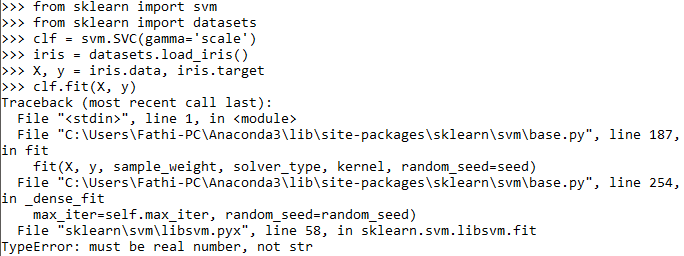
\includegraphics[width=1\textwidth]{figures/fathi/20.PNG}}
\caption{Error Type data, yang harus digunakan number sedangkan isinya 'SCALE' pada gamma}
\label{proses20}

\centerline{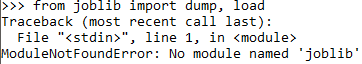
\includegraphics[width=1\textwidth]{figures/fathi/21.PNG}}
\caption{Error no Module found, modul yang dicari tidak ditemukan atau tidak ada 'JOBLIB'}
\label{proses21}
\end{figure}

\item
Error Code and Error Type
\begin{itemize}
\item
Module Not Found
\subitem
module yang dicari tidak ditemukan, karena file yang dicari tidak ada atau belum di instal.

\item
Type Data Error
\subitem
type data yang seharusnya diisikan oleh data number namun diisikan oleh data str/character sedangkan nilai yang bisa dibaca adalah number.
\end{itemize}

\item
Solution
\begin{itemize}
\item
For Module Not Found
\subitem
lakukan instalasi dengan memasukan code berikut untuk download dan instalasi module JOBLIB
\begin{verbatim}
conda install -c anaconda joblib
\end{verbatim}

\item
For Data Type Error
\subitem
ganti isi data menjadi data number, contoh :
\begin{verbatim}
clf = SVC(gamma='scale')
\end{verbatim}
ganti menjadi 
\begin{verbatim}
clf = SVC(gamma=0.5)
\end{verbatim}
\end{itemize}

\end{enumerate}
\end{enumerate}
